% Hlavička
\documentclass{article}

% Preambule - použité balíčky
\usepackage[czech]{babel}		% Čeština (nadpisy, dělení slov, speciální akcenty, jako například ď)
\usepackage{amsmath,amsfonts}	% Matematické symboly a prostředí
\usepackage[utf8]{inputenc}		% Kódování vstupního textu (jinak pouhé ASCII)
\usepackage[unicode]{hyperref}	% Rovnice elegantně odkazy
\usepackage{epsfig}				% Obrázky ve vektorovém formátu EPS
\usepackage{indentfirst}		% České odsazení prvního odstavce 

% Parametry dokumentu
\author{Pavel Stránský}
\title{Kratičké seznámení se s \LaTeX em}

\frenchspacing					% Mezery mezi slovy a mezi větami stejné
								% (v balíčku s češtinou zapnuto automaticky)
\pagestyle{headings}			% Zobrazení záhlaví stránky s názvem sekce a s číslem stránky
								% (kromě první stránky, která má styl trochu jiný)

% Dimenze textu (standardní velikost stránky není příliš ekologická)								
\addtolength{\topmargin}{-0.5cm} 
\addtolength{\textwidth}{1cm}   % Šířka textu
\addtolength{\textheight}{1cm}  % Výška textu
\addtolength{\voffset}{-0.5cm}  % Horní okraj
\addtolength{\hoffset}{-0.5cm}  % Levý okraj
								
% Uživatelská makra
\def\uv#1{\clqq{#1}\crqq}		% Makro pro české uvozovky							
\newcommand{\operator}[1]{\hat{#1}}	% Makro pro operátor na vektorovém prostoru (zápis se stříškou)

% Tělo dokumentu
\begin{document}
	\maketitle					% Vytvoří nadpis
	
	\section{Odstavce}
	\label{sec:odstavce}
		Pro odsazení prvního odstavce je nutné použít balík \textbf{indentfirst}.

		Nezáleží,      kolik
		mezer      vkládáme       ve zdrojovém
		textu
		mezi     slova.
		Jednoduché      zalomení   řádku 
		funguje taky      jako
		mezera.
		Dobrá konvence je psát každou větu na nový řádek.
		Usnadní to práci s verzovacími systémy, jako je třeba \textbf{git}.

		Nový odstavec se vloží pomocí prázdného řádku (nebo pomocí příkazu \verb+\par+).
		
		Ve výjimčených případech lze na nový řádek přejít bez zalomení odstavce.
		K tomu slouží příkazy \verb+\newline+ nebo \verb+\\+.
		\\[2px]
		Druhý jmenovaný příkaz navíc umožňuje použít volitelný parametr udávající šířku dodatečné mezery. 
		Ta může být dokonce i záporná.

		Řádky v dlouhém odstavci se automaticky zalomí. 
		Řádky v dlouhém odstavci se automaticky zalomí. 
		Řádky v dlouhém odstavci se automaticky zalomí. 
		Řádky v dlouhém odstavci se automaticky zalomí. 
		Řádky v dlouhém odstavci se automaticky zalomí. 
		
		\LaTeX{} automaticky dělí slova.
		\LaTeX{} automaticky dělí slova.
		\LaTeX{} automaticky dělí slova.
		\LaTeX{} automaticky dělí slova.
		\LaTeX{} automaticky dělí slova.
		
		Po jednopísmenných předložkách a spojkách dáváme nedělitelné mezery pomocí symbolu~\~{}.
		Rovněž například mezi dnem a měsícem u data.
		Vypadá to líp.

	\section{Uvozovky}
		Různé druhy uvozovek: \uv{české} (vytvořené pomocí makra) nebo ``English''.

	\section{Pomlčky}
		% Spojovník a krátká pomlčka (pro intervaly)
		Půjde-li to, sejdeme se v 10--16~hodin.
		% Dlouhá pomlčka - interpunkce, v anglickém textu bez mezer
		Důležité je, abychom v textu --- to je to, co teď píšeme --- správně používali pomlčky.
		V anglickém jazyce se používají trochu jinak než v českém.
		Pozor, znaménko $-3$ není pomlčka. 
		Vysází se v matematickém režimu.

	\section{Výpustky}
		To máte cihly, hřebíky, šrouby, matky, vruty, \ldots

	\section{Háčky, čárky a další ozdůbky}
	\label{sec:akcenty}
		H\^otel,
		na\"\i ve, 
		\'el\`eve, 
		sm\o rrebr\o d, 
		!‘Se\~norita!,	
		Sch\"onbrunner Schlo\ss stra\ss e,
		pot\r u\v cek
		
		\`a \'a \^a \r a \v a \"a  \H a
		\~a \=a \b a \.a \u a \t{aa} \c a \d a

		\i \j
		
	\section{Řezy písma a velikost písma}
		Kromě běžného normálního stojatého netučného písma typu antikva (roman) lze použít i \textbf{tučné písmo}, \textit{italiku (kurzívu)}, \textsf{bezpatkové písmo (grotesk)}, \textsc{kapitálky} nebo \texttt{strojové písmo}.
		Řezy písem lze \textit{\textbf{kombinovat}}.
		Pro velikost písem slouží příkazy
		{\tiny\verb+\tiny+}, 
		{\scriptsize\verb+\scriptsize+},
		{\footnotesize\verb+\footnotesize+},
		{\small\verb+\small+},
		{\normalsize\verb+\normalsize+},
		{\large\verb+\large+},
		{\Large\verb+\Large+},
		{\LARGE\verb+\LARGE+},
		{\huge\verb+\huge+} a
		{\Huge\verb+\Huge+}.

		Jako u všeho platí: různá písma v jednom textu používejte s mírou, systematicky a radši méně než více.

	\section{Nadpisy}
		Důležité je nejen, jak text vypadá, ale i jak je strukturovaný.
		\subsection{Podsekce}
			\subsubsection{Podpodsekce}	
				Podsekce a podpodsekce jsou číslované.
				Hlubší úrovně Odstavec a Pododstavec číslované nejsou.
				\paragraph{Odstavec}
					Sem by se hodilo něco duchaplného.
					\subparagraph{Pododstavec}

	\section{Křížové odkazy}
	V sekci~\ref{sec:akcenty} na straně~\pageref{sec:akcenty} jsou příklady veškeré diakritiky, kterou~\LaTeX{} zná.
	Rovnice~\eqref{eq:Brouncker} se mi obzvlášť líbí.
	K pojmenování návěští odkazovaných objektů se používá konvence, kdy první písmena obsahují typ objektu (sekce, obrázek, rovnice, tabulka, \ldots).
	Jako vše v \LaTeX{}u, i ve jménech návěští záleží na velikosti písem.
	V pojmenování lze použít i diakritiku.
	
	\section{Poznámky pod čarou}
	Poznámka pod čarou\footnote{V některých stylech ani čára nemusí být přítomna.} se píše velmi jednoduše.

	\section{Zvýraznění textu a různá písma}
	\emph{Důležité myšlenky} je potřeba zvýraznit.
	V tištěném textu se zdůrazněněné části nepodtrhávají, nýbrž sázejí se kurzívou.
	
	\section{Výčty}
	Výčty mohou být buď
	\begin{enumerate}
		\item číslované
	\end{enumerate}
	nebo
	\begin{itemize}
		\item nečíslované.
	\end{itemize}
	\LaTeX{} zná i další typy výčtů.
	Zde budeme tajemní a nezmíníme je.	

	\section{Rovnice}
	V textu se zapisují pomocí znaku dolaru: $a^2+b^2=c^2$.
	Na speciální řádku se hodí složitější rovnice, jako je třeba Leibnizova řada pro výpočet čísla $\pi$:
	\begin{equation}
		\frac{\pi}{4}=\sum_{k=1}^{\infty}\frac{(-1)^{k+1}}{2k-1}
			=1-\frac{1}{3}+\frac{1}{5}-\dotsb.
	\end{equation}
	Pro číslo $\pi$ existují i jiné formule, třeba tato Newtonova
	\begin{equation}
		\pi=\frac{3}{4}\sqrt{3}+24\int_{0}^{\frac{1}{4}}\sqrt{x-x^2}dx,
	\end{equation}
	Vi\`etova daná jako nekonečný součin vnořených odmocnin
	\begin{equation}
		\frac{2}{\pi}=\sqrt{\frac{1}{2}}\sqrt{\frac{1}{2}+\frac{1}{2}\sqrt{\frac{1}{2}}}\sqrt{\frac{1}{2}+\frac{1}{2}\sqrt{\frac{1}{2}+\frac{1}{2}\sqrt{\frac{1}{2}}}}\dotsb
	\end{equation}
	nebo Brounckerova pomocí řetězových zlomků~\cite{Beckmann1998}
	\begin{equation}
		\label{eq:Brouncker}
		\frac{4}{\pi}=1+\frac{1^2}{2+\frac{3^2}{2+\frac{5^2}{2+\frac{7^2}{2+\dotsb}}}}.
	\end{equation}
	
	Mezery je v matematických textech potřeba ošetřit zvlášť:
	\begin{equation}
		\forall x\in\mathbb{R}\qquad x^{2}\geq0 \quad\textrm{(platí skoro vždy)}.
	\end{equation}
	
	Jelikož proměnné se sází kurzívou, zatímco názvy funkcí nikoliv,
	jsou v \LaTeX u speciální příkazy pro funkce:
	\begin{equation}
		\sin^{2}x+\cos^2{x}=1.
	\end{equation}
	
	Velikost závorek je nejlepší nechat přímo na \LaTeX u:
	\begin{equation}
		f(x)=\left[\sum_{n=1}^{\infty}\frac{\left(x^2-1\right)^n}{n}\right]^2.
	\end{equation}
	
	Matematická prostředí umožňují i zápis více rovnic zarovnaných úhledně pod sebe.
	Například objem a povrch koule se spočítají pomocí výrazů
	\begin{align}
		S&=4\pi R^{2},\\
		V&=\frac{4}{3}\pi R^{3},
	\end{align}
	kde $R$ je poloměr koule a $\pi$ je Ludolfovo číslo, uvedené níže v tabulce~\ref{tab:tabulka}.
	Pozor: I~když se rovnice píší na samostatný řádek, jsou stále součástí textu.
	Je tedy nutné dodržet správnou interpunkci.
	Často se v tom chybuje.
	
	Rovnici, která si zaslouží vlastní řádek, ale nikoliv své číslo, vytvoříme pomocí ohvězdičkovaného názvu prostředí:
	\begin{equation*}
		\nabla\phi=0.
	\end{equation*}

	Pro všemožné symboly je dobré konzultovat bohaté zdroje na webu,
	například několikasetstránkový dokument~\cite{SymbolList2017}. 
	
	\section{Obrázky}
		% htbp udává, že nejprve se LaTeX snaží umístit objekt zde (here).
		% Pokud se mu to nepodaří, pokusí se použít začátek stránky, pak konec stránky a 
		% nakonec samostatnou stránku. 
		% Vykřičník mu dovolí být "agresivnější" a přimhouřit oči nad některými typografickými
		% pravidy.
		\begin{figure}[!htbp]
			\centering
			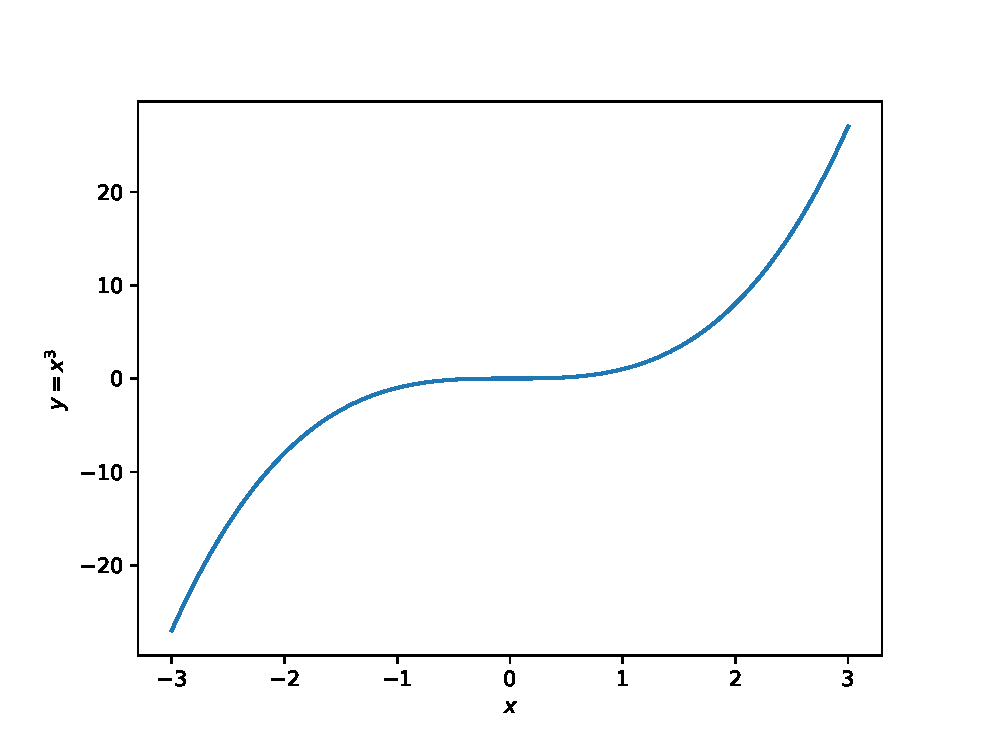
\includegraphics[width=0.8\linewidth]{kubik.eps}
			\caption{Kubická funkce $y=x^3$.}
			\label{fig:bandf}
		\end{figure}
		Obrázky se doporučuje používat jako plovoucí objekty, což znamená, že se neobjeví přesně tam, kde je vložíme, nýbrž tam, kam nejlépe padnou a kde splní všechna typografická pravidla.

	\section{Tabulky}
		Stejné pravidlo jako pro obrázky platí i pro tabulky, jen prostředí se místo \verb+\figure+ nazývá \verb+\table+.
		\begin{table}[b]
			\centering
			\begin{tabular}{|c || r l |} 
			\hline
				Na střed & Doprava & Doleva \\				
			\hline\hline
				Ludolf & 3.14 & $\pi$ \\
				Euler & 2.72 & $e$ \\
				Euler-Mascheroni & 0.577 & $\gamma=\lim_{n\rightarrow\infty}\left(-\log n+\sum_{k=1}^{n}\frac{1}{k}\right)$ \\
			\hline
			\end{tabular}
			\caption{Tři zajímavé matematické konstanty.}
			\label{tab:tabulka}
		\end{table}
		V tabulce~\ref{tab:tabulka} umístěné ke konci stránky jsou tři zajímavé konstanty.

		\section{Závěr}
		K úplně základnímu seznámení se s psaním v \LaTeX u tento text může stačit.
		Rozhodně doporučuji přečíst si nějaký trochu podrobnější návod, jakým je například~\cite{UvodLaTeX1998}.

	\begin{thebibliography}{99}
		\bibitem{SymbolList2017} S. Pakin, \href{http://tug.ctan.org/info/symbols/comprehensive/symbols-a4.pdf}{The comprehensive \LaTeX{} Symbol List} (2017).
		\bibitem{UvodLaTeX1998} T. Oetiker, H, Partl, I. Hyna, E. Schlegl, M. Kočer, P. Sýkora,
			\href{http://www.penguin.cz/~kocer/texty/lshort2e/lshort2e-cz.pdf}{Ne příliš stručný návod do systému \LaTeXe} (1998).
		\bibitem{Beckmann1998} P. Beckmann, \textit{Historie čísla $\pi$} (Academia Praha, 1998).
	\end{thebibliography}

	% Vypíše obsah
	\tableofcontents

	% Vypíše seznam obrázků
	\listoffigures

	% Vypíše seznam tabulek
	\listoftables

\end{document}
% Vše, co je za tímto příkazem, je ignorováno.

Text, který se nezobrazí.